\section{Resultados}
\label{sec:resultados}

Os resultados correspondem ao cenário ambiental descrito na seção~\ref{sec:dados}. A leitura parte da rede completa $W$ para distinguir volume e concentração das atribuições e identificar as contrapartes que compõem os perfis setoriais. Em seguida, examina quais relações o filtro destaca e quanto dessa composição permanece representado no backbone $B$.

\subsection{Contas ambientais, volume e concentração}

As duas contas pela ótica da produção $c$ e da demanda $u$ totalizam 683,70 mil Gg de CO\textsubscript{2}, dos quais 392,92 mil Gg estão na diagonal de $F$ e 290,78 mil Gg nas relações entre atividades distintas em $W$. A igualdade entre os totais pela produção e pela demanda decorre da identidade contábil. A parcela intersetorial permite examinar como as mesmas emissões conectam origens e produtos finais, enquanto a diagonal situa o volume atribuído aos produtos finais da própria atividade emissora.

A rede completa tem 67 nós e 4\,290 arestas, com densidade de 97,01\%. Serviços domésticos (9700) é o único nó isolado: sua conta permanece na diagonal de $F$. As outras 66 atividades estão ligadas entre si nas duas direções, com graus iguais a 65. A presença de relações é compatível com a incorporação dos requisitos indiretos em $F$ e pouco distingue os perfis setoriais. O conteúdo desses perfis precisa ser examinado pela distribuição dos pesos.

Entre as 66 atividades conectadas, o número efetivo de contrapartes, $D_2$, varia de 1,58 a 25,04 destinos nas saídas e de 2,13 a 22,10 origens nas entradas; as medianas são 11,50 e 13,93, respectivamente. Embora todas tenham 65 ligações em cada direção, as emissões se concentram de maneira distinta entre as contrapartes. Para compreender sua distribuição entre atividades emissoras e setores de produtos finais, é necessário considerar tanto os volumes atribuídos, medidos pelas forças, quanto sua concentração, expressa por $D_2$. Os painéis A e B da Figura~\ref{fig:indicadores-resultados} permitem examinar essa relação nas atividades com as oito maiores forças de saída ou de entrada em $W$.

Energia (3500) e água, esgoto e resíduos (3680) apresentam as duas maiores forças de saída, com volumes semelhantes: 31,32 e 31,23 mil Gg, respectivamente. Esses volumes, porém, distribuem-se de maneira diferente entre os setores de produtos finais. O número efetivo de destinos é de 20,79 em energia e de 9,88 em água/resíduos, indicando maior concentração das atribuições desta última atividade. Assim, atividades com volumes semelhantes de emissões intersetoriais podem diferir quanto à concentração dessas emissões entre os destinos.

A Tabela~\ref{tab:contas-energia-construcao} relaciona os volumes intersetoriais da Figura~\ref{fig:indicadores-resultados} às contas completas de três atividades. Energia e água/resíduos são mantidas na comparação por apresentarem as duas maiores forças de saída, com volumes semelhantes e concentrações distintas. Construção, com a terceira maior força de entrada, permite examinar a perspectiva do destino e o peso das emissões de outras origens no total atribuído aos seus produtos finais.

\clearpage
\begin{figure}[p]
\centering
\caption{Forças e concentração nas atividades com as oito maiores forças de saída ou de entrada na rede completa, Brasil, 2015.}
\label{fig:indicadores-resultados}
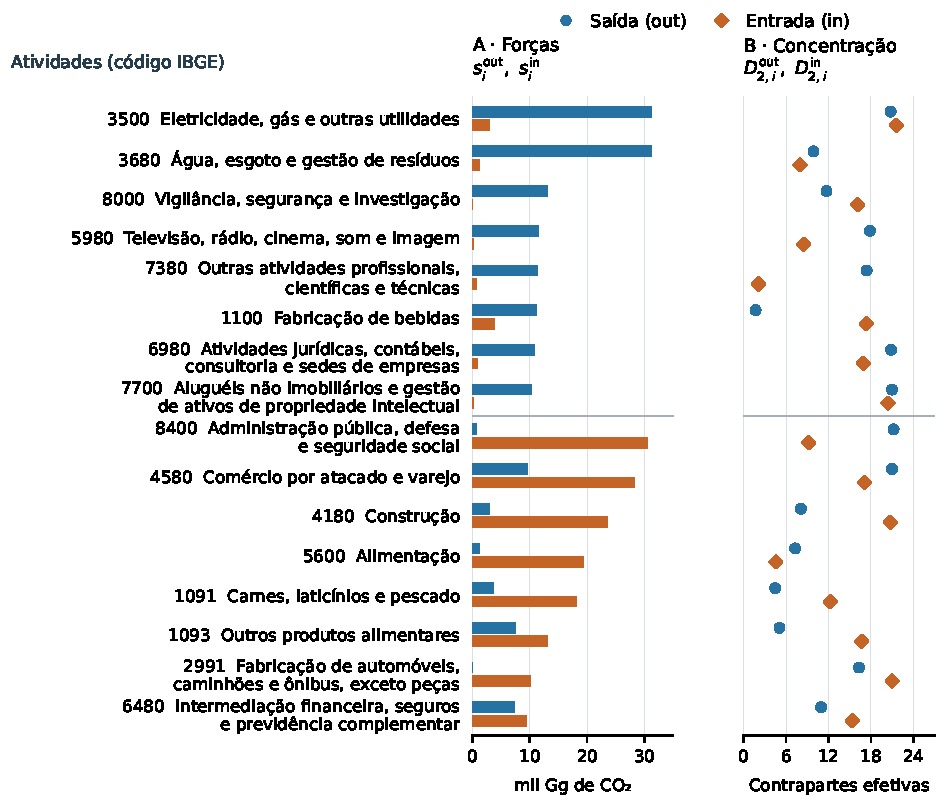
\includegraphics[width=\textwidth,height=0.94\textheight,keepaspectratio]{figuras/indicadores_rede_completa.pdf}
\begin{notas}
Nota: A figura apresenta as 16 atividades que compõem a união das oito maiores forças de saída e das oito maiores forças de entrada da rede completa $W$. Essa rede relaciona as emissões geradas em cada atividade à demanda final dos produtos de outras atividades, considerando apenas atribuições entre atividades distintas. O azul representa a perspectiva de saída, na qual as emissões da atividade indicada são atribuídas aos produtos finais de outras atividades. O laranja representa a perspectiva de entrada, na qual emissões geradas em outras atividades são atribuídas aos produtos finais da atividade indicada.
\par
No painel A, a força de saída, $s_i^{\mathrm{out}}$, mede o volume de emissões próprias atribuído aos produtos finais de outras atividades. A força de entrada, $s_i^{\mathrm{in}}$, mede o volume de emissões de outras atividades atribuído aos produtos finais da atividade indicada. Os volumes são expressos em mil Gg de CO\textsubscript{2}; cada Gg corresponde a mil toneladas.
\par
No painel B, a concentração desses volumes é representada pelo número efetivo de contrapartes, $D_2$, calculado como o inverso do índice de concentração $Y$. O número efetivo expressa quantas contrapartes com participações iguais produziriam a concentração observada. Na saída, as contrapartes são os destinos das atribuições, representados por $D_{2,i}^{\mathrm{out}}$; na entrada, são as origens emissoras, representadas por $D_{2,i}^{\mathrm{in}}$. Quanto menor o número efetivo de contrapartes, maior a concentração das emissões.
\par
Acima da linha horizontal estão as oito atividades com maiores forças de saída; abaixo estão as oito atividades com maiores forças de entrada. Em cada grupo, as atividades aparecem em ordem decrescente da força utilizada na seleção. Os rótulos apresentam os códigos do IBGE e os nomes abreviados das atividades.
\end{notas}
\end{figure}
\clearpage

\begin{table}[!ht]
\centering
\caption{Decomposição das contas de emissões de CO\textsubscript{2} pela produção e pela demanda em energia, água/resíduos e construção, Brasil, 2015 (mil Gg de CO\textsubscript{2}).}
\label{tab:contas-energia-construcao}
\small
\begin{tabular*}{\textwidth}{@{}l@{\extracolsep{\fill}}rrrrrr@{}}
\toprule
\shortstack[l]{Atividade\\(código IBGE)} & \shortstack{Diagonal\\$F_{ii}$} & \shortstack{Saída\\externa\\$s_i^{\mathrm{out}}$} & \shortstack{Entrada\\externa\\$s_i^{\mathrm{in}}$} & \shortstack{Produção\\$c_i$} & \shortstack{Demanda\\$u_i$} & \shortstack{Saldo\\$u_i-c_i$} \\
\midrule
Energia (3500) & 25,30 & 31,32 & 2,92 & 56,62 & 28,23 & $-28,39$ \\
Água/resíduos (3680) & 20,57 & 31,23 & 1,16 & 51,80 & 21,74 & $-30,07$ \\
Construção (4180) & 35,91 & 2,93 & 23,48 & 38,84 & 59,40 & 20,56 \\
\bottomrule
\end{tabular*}
\begin{notas}
Nota: O recorte abrange emissões da produção nacional associadas à demanda doméstica e às exportações, excluindo emissões estrangeiras. Cada linha corresponde à atividade $i$. Produção ($c_i$) contabiliza as emissões na atividade em que ocorrem; demanda ($u_i$) reúne as emissões diretas e indiretas atribuídas aos produtos finais da atividade. A diagonal ($F_{ii}$) corresponde às emissões geradas na própria atividade e atribuídas aos seus produtos finais, incluindo requisitos indiretos. A força de saída, ou saída externa ($s_i^{\mathrm{out}}$), mede as emissões próprias atribuídas aos produtos finais de outras atividades. A força de entrada, ou entrada externa ($s_i^{\mathrm{in}}$), mede as emissões de outras atividades atribuídas aos produtos finais da atividade indicada. Assim, $c_i=F_{ii}+s_i^{\mathrm{out}}$ e $u_i=F_{ii}+s_i^{\mathrm{in}}$; o saldo $u_i-c_i=s_i^{\mathrm{in}}-s_i^{\mathrm{out}}$ é entrada menos saída externa. Diferenças residuais nas somas decorrem do arredondamento.
\par
Seleção: energia e água/resíduos apresentam as duas maiores saídas externas; construção, a terceira maior entrada externa entre as 67 atividades. São casos ilustrativos. Nomes completos: energia elétrica, gás natural e outras utilidades (3500); água, esgoto e gestão de resíduos (3680).
\par
Dados: Matriz de Insumo-Produto do IBGE de 2015 e coeficientes de emissão interpolados de \textcite{sanguinetAzzoni2024}.
\end{notas}
\end{table}

Em energia e água/resíduos, as emissões próprias atribuídas a outros produtos finais superam as emissões de outras origens atribuídas aos seus produtos finais. Por isso, suas contas pela demanda são menores que as contas pela produção; na construção, ocorre o inverso. A diagonal, comum às duas contas, permite situar o peso dessas relações intersetoriais. Na construção, 35,91 mil Gg são gerados na própria atividade e atribuídos aos seus produtos finais, equivalentes a 92,5\% da conta pela produção. Portanto, a pequena saída externa não implica um pequeno volume de emissões próprias. Já na conta pela demanda da construção, as emissões de outras atividades representam 39,5\% do total, enquanto os 60,5\% restantes correspondem à diagonal.

A distribuição das emissões entre origens e produtos finais combina, portanto, atribuições dentro da própria atividade e relações entre atividades distintas. A tabela distingue o volume dessas parcelas; a composição dos perfis, examinada a seguir, identifica quais origens e destinos participam das relações intersetoriais.





\subsection{Composição dos perfis de atribuição}
\label{sec:composicao-perfis}

O contraste de concentração entre energia e água/resíduos na Figura~\ref{fig:indicadores-resultados} envolve participações distintas de destinos compartilhados. Comércio, administração pública e construção aparecem entre os cinco maiores destinos de ambas as atividades (Tabela~\ref{tab:contrapartes-completas}). Entretanto, administração pública reúne 27,22\% das saídas de água/resíduos e 8,16\% das saídas de energia. Essa diferença ajuda a interpretar por que volumes intersetoriais semelhantes se distribuem de forma mais concentrada no primeiro perfil. O peso de administração pública identifica as emissões atribuídas aos produtos finais desse setor, incluindo seus requisitos diretos e indiretos de produção; não corresponde a uma medida das compras diretas do governo junto às atividades emissoras.

\begin{table}[p]
\centering
\caption{Cinco maiores contrapartes nas saídas de energia e de água/resíduos e nas entradas de construção, antes do filtro, Brasil, 2015.}
\label{tab:contrapartes-completas}
\small
\begin{tabular*}{\textwidth}{@{}>{\raggedright\arraybackslash}p{0.57\textwidth}@{\extracolsep{\fill}}rr@{}}
\toprule
Contraparte (código IBGE) & \shortstack{Emissões\\(mil Gg de CO\textsubscript{2})} & \shortstack{Participação no\\volume externo (\%)} \\
\midrule
\multicolumn{3}{@{}l}{\textit{Saídas de energia (3500): destinos dos produtos finais}} \\
Comércio (4580) & 4,224 & 13,49 \\
Administração pública, defesa e seguridade social (8400) & 2,556 & 8,16 \\
Construção (4180) & 2,263 & 7,23 \\
Abate e produtos de carne, laticínio e pesca (1091) & 1,930 & 6,16 \\
Agricultura (0191) & 1,693 & 5,41 \\
Demais 60 destinos & 18,650 & 59,55 \\
Total externo ($s_{3500}^{\mathrm{out}}$) & 31,317 & 100,00 \\
\midrule
\multicolumn{3}{@{}l}{\textit{Saídas de água/resíduos (3680): destinos dos produtos finais}} \\
Administração pública, defesa e seguridade social (8400) & 8,501 & 27,22 \\
Comércio (4580) & 2,964 & 9,49 \\
Saúde privada (8692) & 1,672 & 5,35 \\
Saúde pública (8691) & 1,621 & 5,19 \\
Construção (4180) & 1,592 & 5,10 \\
Demais 60 destinos & 14,880 & 47,65 \\
Total externo ($s_{3680}^{\mathrm{out}}$) & 31,230 & 100,00 \\
\midrule
\multicolumn{3}{@{}l}{\textit{Entradas de construção (4180): origens emissoras}} \\
Produtos de minerais não metálicos (2300) & 2,959 & 12,60 \\
Energia elétrica, gás natural e outras utilidades (3500) & 2,263 & 9,64 \\
Água, esgoto e gestão de resíduos (3680) & 1,592 & 6,78 \\
Comércio (4580) & 1,240 & 5,28 \\
Produtos de metal, exceto máquinas e equipamentos (2500) & 1,037 & 4,42 \\
Demais 60 origens & 14,393 & 61,29 \\
Total externo ($s_{4180}^{\mathrm{in}}$) & 23,484 & 100,00 \\
\bottomrule
\end{tabular*}
\begin{notas}
Nota: cada relação atribui emissões da produção nacional a um setor de produtos finais, incluindo requisitos diretos e indiretos para a demanda doméstica e as exportações; emissões estrangeiras são excluídas. Nas saídas, a atividade indicada no título do bloco é a origem emissora $i$, e cada contraparte é um destino $j$: a emissão é $W_{ij}$, e a participação é $100W_{ij}/s_i^{\mathrm{out}}$. Nas entradas, a atividade indicada é o destino $i$, e cada contraparte é uma origem emissora $j$: a emissão é $W_{ji}$, e a participação é $100W_{ji}/s_i^{\mathrm{in}}$. As forças $s_i^{\mathrm{out}}$ e $s_i^{\mathrm{in}}$ são os volumes externos totais de cada direção. A diagonal, que atribui emissões aos produtos finais da própria atividade emissora, é excluída; os percentuais não usam as contas completas pela produção ou pela demanda.
\par
Seleção: energia e água/resíduos são as duas maiores forças de saída; construção é a terceira maior força de entrada entre as 67 atividades. Cada perfil completo tem 65 contrapartes com atribuição positiva. Mostram-se as cinco maiores, em ordem decrescente de emissão, e as demais 60 agregadas, sem filtragem das relações. Energia $\rightarrow$ construção e água/resíduos $\rightarrow$ construção aparecem nas perspectivas da origem e do destino, com o mesmo volume e denominadores distintos; cada relação deve ser contada apenas uma vez nos totais da rede. Nomes abreviados: energia corresponde a energia elétrica, gás natural e outras utilidades; água/resíduos, a água, esgoto e gestão de resíduos. Diferenças residuais nas somas decorrem do arredondamento dos valores calculados no notebook.
\par
Dados: Matriz de Insumo-Produto do IBGE de 2015 e coeficientes de emissão interpolados de \textcite{sanguinetAzzoni2024}.
\end{notas}
\end{table}
\clearpage

A comparação com construção mostra que uma concentração semelhante pode corresponder a papéis distintos na atribuição das emissões. Na Figura~\ref{fig:indicadores-resultados}, as saídas de energia e as entradas de construção têm números efetivos próximos, ambos de aproximadamente 20,8 contrapartes. Energia distribui emissões próprias entre produtos finais de outras atividades; construção reúne emissões geradas em diferentes origens. Na Tabela~\ref{tab:contrapartes-completas}, produtos de minerais não metálicos, energia e produtos de metal estão entre as principais origens da construção, mas as cinco maiores origens, em conjunto, representam apenas 38,71\% das entradas externas. A parcela intersetorial de 39,5\% da conta pela demanda, identificada na seção anterior, envolve, portanto, uma composição que ultrapassa as principais atividades produtoras de materiais e de energia. Mesmo a atividade de produtos de minerais não metálicos, a maior origem externa, representa 12,60\% das entradas externas e aproximadamente 5,0\% da conta completa pela demanda da construção.

Os perfis também permitem reconhecer as duas perspectivas de uma mesma relação. Construção aparece entre os principais destinos de energia e água/resíduos, que, por sua vez, estão entre as principais origens das entradas de construção. Energia $\rightarrow$ construção representa 7,23\% das saídas externas de energia e 9,64\% das entradas externas de construção. O volume atribuído é o mesmo, mas sua participação muda conforme se examina a distribuição das emissões da origem ou a composição recebida pelo destino. Assim, a descrição das relações exige considerar as duas perspectivas: a posição de uma atividade como origem não determina o peso de cada destino, e a composição de um destino não informa, por si só, quanto ele representa para cada origem. Essa distinção orienta a leitura do filtro nas seções seguintes, em que a seleção de uma ligação é avaliada separadamente na origem e no destino.

\subsection{Seleção das relações e limites de cobertura}

As participações examinadas na seção~\ref{sec:composicao-perfis} mostram que uma relação pode ter importâncias distintas para a origem e o destino. O filtro de disparidade considera essas duas perspectivas ao selecionar as relações do backbone, mantendo as contas e os perfis completos como referência. Para interpretar a distribuição das emissões nessa representação selecionada, é necessário verificar quanto do volume permanece e se a cobertura é semelhante entre atividades e direções.

Em $\alpha=0{,}05$, apenas 13,40\% das relações preservam 70,69\% das emissões intersetoriais (Tabela~\ref{tab:sensibilidade-backbone}). Uma parcela relativamente pequena das relações reúne, portanto, grande parte do volume. Essa redução também omite 29,31\% das emissões entre atividades distintas, que continuam presentes na rede completa e nas contas ambientais. O backbone permite examinar relações selecionadas, mas não substitui a composição completa descrita nas seções anteriores.

A cobertura global, entretanto, não descreve igualmente os dois papéis de uma atividade. A Figura~\ref{fig:indicadores-backbone} mantém as atividades da Figura~\ref{fig:indicadores-resultados} e mostra que, em energia, a seleção representa 99,2\% das saídas, mas apenas 42,1\% das entradas. Assim, o backbone permite acompanhar quase todo o volume de emissões próprias atribuído a outros produtos finais, enquanto deixa de representar a maior parte das emissões de outras origens atribuídas aos produtos finais de energia. Uma lista curta de origens selecionadas não basta para caracterizar a concentração desse perfil: o grau conta relações retidas, a cobertura mede seu alcance em volume e o número efetivo descreve a concentração na rede completa.

A matriz da Figura~\ref{fig:matriz-backbone} acrescenta a localização e o volume das relações selecionadas. Suas linhas permitem acompanhar os destinos das emissões de energia e água/resíduos; a coluna de construção reúne as origens retidas na atribuição aos produtos finais desse setor. Essas perspectivas situam no conjunto das atividades as relações examinadas na Tabela~\ref{tab:contrapartes-completas}. As diferenças de tonalidade mostram que a seleção por importância relativa admite relações de volumes absolutos distintos. Por isso, uma célula mais escura indica maior volume atribuído à relação, mas não maior concentração do perfil nem maior importância relativa para suas duas extremidades.

\begin{table}[htbp]
\centering
\caption{Relações e emissões preservadas pelo filtro de disparidade em diferentes limiares, Brasil, 2015.}
\label{tab:sensibilidade-backbone}
\small
\begin{tabular*}{\textwidth}{@{}l@{\extracolsep{\fill}}rrr@{}}
\toprule
Rede ou limiar & \shortstack{Relações\\n (\%)} & \shortstack{Emissões retidas\\(mil Gg de CO\textsubscript{2})} & \shortstack{Cobertura\\(\%)} \\
\midrule
Sem filtro ($W$) & 4\,290 (100,00) & 290,78 & 100,00 \\
$\alpha=0{,}01$ & 338 (7,88) & 166,88 & 57,39 \\
$\alpha=0{,}05$ (referência) & 575 (13,40) & 205,55 & 70,69 \\
$\alpha=0{,}10$ & 755 (17,60) & 224,92 & 77,35 \\
\bottomrule
\end{tabular*}
\begin{notas}
Nota: cada relação atribui emissões geradas em uma atividade brasileira aos produtos finais de outra, incluindo requisitos diretos e indiretos para a demanda doméstica e as exportações. Emissões estrangeiras e atribuições aos produtos finais da própria atividade emissora (diagonal) são excluídas. A rede completa $W$, sem filtro, contém 4\,290 relações e 290,78 mil Gg de CO\textsubscript{2}. Os percentuais de relações usam como denominador as relações de $W$; a cobertura é a porcentagem das emissões intersetoriais de $W$ preservada em cada seleção. Valores são calculados antes do arredondamento; cada Gg corresponde a mil toneladas.
\par
O parâmetro $\alpha$ é o limiar das probabilidades de cauda do modelo nulo do filtro de disparidade: valores maiores tornam a seleção mais permissiva. Pela regra OU, basta a relação ser selecionada na perspectiva da origem ou do destino. Cada filtro é aplicado à mesma rede completa, sem recalcular as participações após a seleção. Os pesos originais das relações preservadas são mantidos, e as contas completas pela produção e pela demanda não mudam. Todos os casos mantêm 67 atividades, uma isolada e um componente de 66 atividades conectadas quando se desconsidera a direção das relações. O limiar de referência não é considerado ótimo.
\par
Dados: Matriz de Insumo-Produto do IBGE de 2015 e coeficientes de emissão interpolados de \textcite{sanguinetAzzoni2024}.
\end{notas}
\end{table}


A sensibilidade ao limiar delimita essa leitura. Na Tabela~\ref{tab:sensibilidade-backbone}, aumentar $\alpha$ amplia as relações e o volume representados, mas as coberturas agregadas não demonstram estabilidade de cada contraparte ou posição setorial. Mesmo com um componente de 66 atividades nos três limiares, a quantidade de relações e os postos por grau mudam, conforme os diagnósticos do \ref{anexo:diagnosticos}. Mantém-se $\alpha=0{,}05$ como referência convencional. A leitura do backbone precisa, portanto, combinar os volumes completos, a cobertura de cada perfil e a perspectiva responsável pela seleção, examinada a seguir.

\clearpage
\begin{figure}[p]
\centering
\caption{Graus e coberturas do backbone nas atividades com as oito maiores forças de saída ou de entrada na rede completa, Brasil, 2015.}
\label{fig:indicadores-backbone}
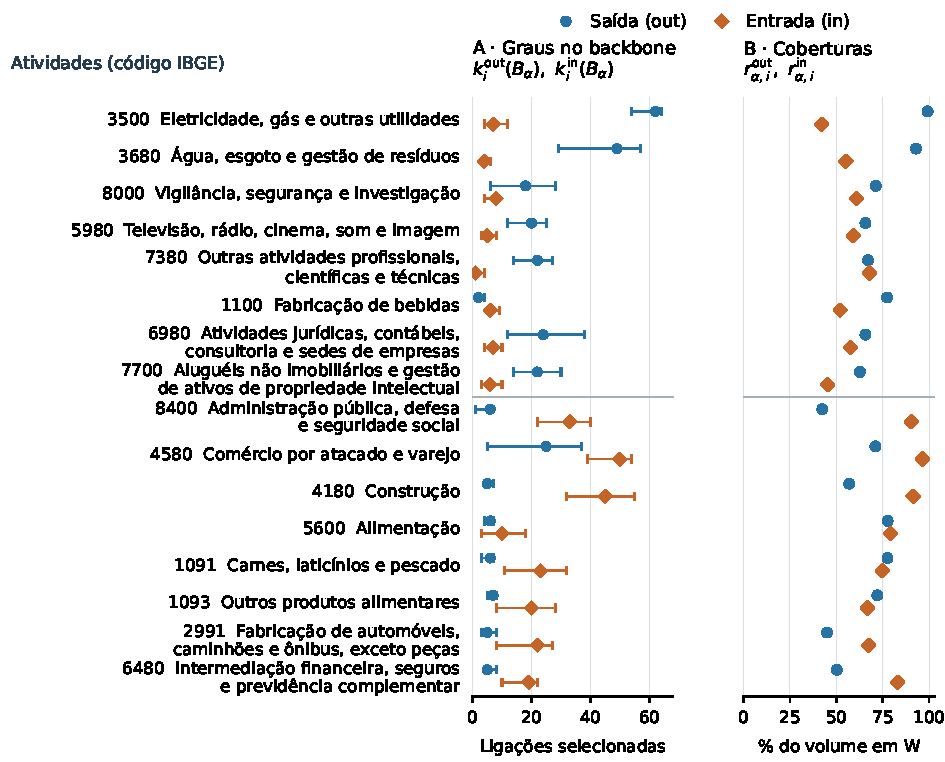
\includegraphics[width=\textwidth,height=0.94\textheight,keepaspectratio]{figuras/indicadores_backbone.pdf}
\begin{notas}
Nota: A figura apresenta os graus e as coberturas do backbone para as 16 atividades que compõem a união das oito maiores forças de saída e das oito maiores forças de entrada da rede completa $W$. A seleção das atividades é feita pelas forças em $W$, antes da filtragem. O backbone $B_\alpha$ é obtido pelo filtro de disparidade, que seleciona ligações com participações excepcionalmente altas na força da origem ou do destino em comparação com uma distribuição aleatória de referência. Os pesos originais das ligações selecionadas são preservados.
\par
O azul representa as ligações de saída da atividade indicada para outros setores de produtos finais. O laranja representa as ligações de entrada, pelas quais emissões de outras atividades são atribuídas aos produtos finais da atividade indicada.
\par
No painel A, os graus de saída e de entrada, $k_i^{\mathrm{out}}(B_\alpha)$ e $k_i^{\mathrm{in}}(B_\alpha)$, indicam o número de ligações preservadas em cada direção. Os pontos mostram os graus obtidos com $\alpha=0{,}05$. As barras horizontais abrangem os graus obtidos entre $\alpha=0{,}01$ e $\alpha=0{,}10$ e mostram a sensibilidade do número de ligações ao limiar do filtro; não são intervalos de confiança.
\par
No painel B, as coberturas de saída e de entrada, $r_{\alpha,i}^{\mathrm{out}}$ e $r_{\alpha,i}^{\mathrm{in}}$, mostram a porcentagem do volume de emissões de cada atividade e direção preservada no backbone para $\alpha=0{,}05$. Cada cobertura compara a soma dos pesos das ligações selecionadas com a força correspondente na rede completa $W$. Assim, o grau informa quantas ligações permanecem, enquanto a cobertura informa quanto do volume original essas ligações representam. Ambos se referem à seleção; o número efetivo de contrapartes da Figura~\ref{fig:indicadores-resultados} caracteriza a concentração dos pesos na rede completa.
\par
Acima da linha horizontal estão as oito atividades com maiores forças de saída em $W$; abaixo estão as oito atividades com maiores forças de entrada em $W$. Em cada grupo, as atividades aparecem em ordem decrescente da força utilizada na seleção. Os rótulos apresentam os códigos do IBGE e os nomes abreviados das atividades.
\end{notas}
\end{figure}
\clearpage
\begin{landscape}
\begin{figure}[p]
\centering
\caption{Emissões de CO\textsubscript{2} nas relações selecionadas pelo filtro de disparidade, $\alpha=0{,}05$, Brasil, 2015.}
\label{fig:matriz-backbone}
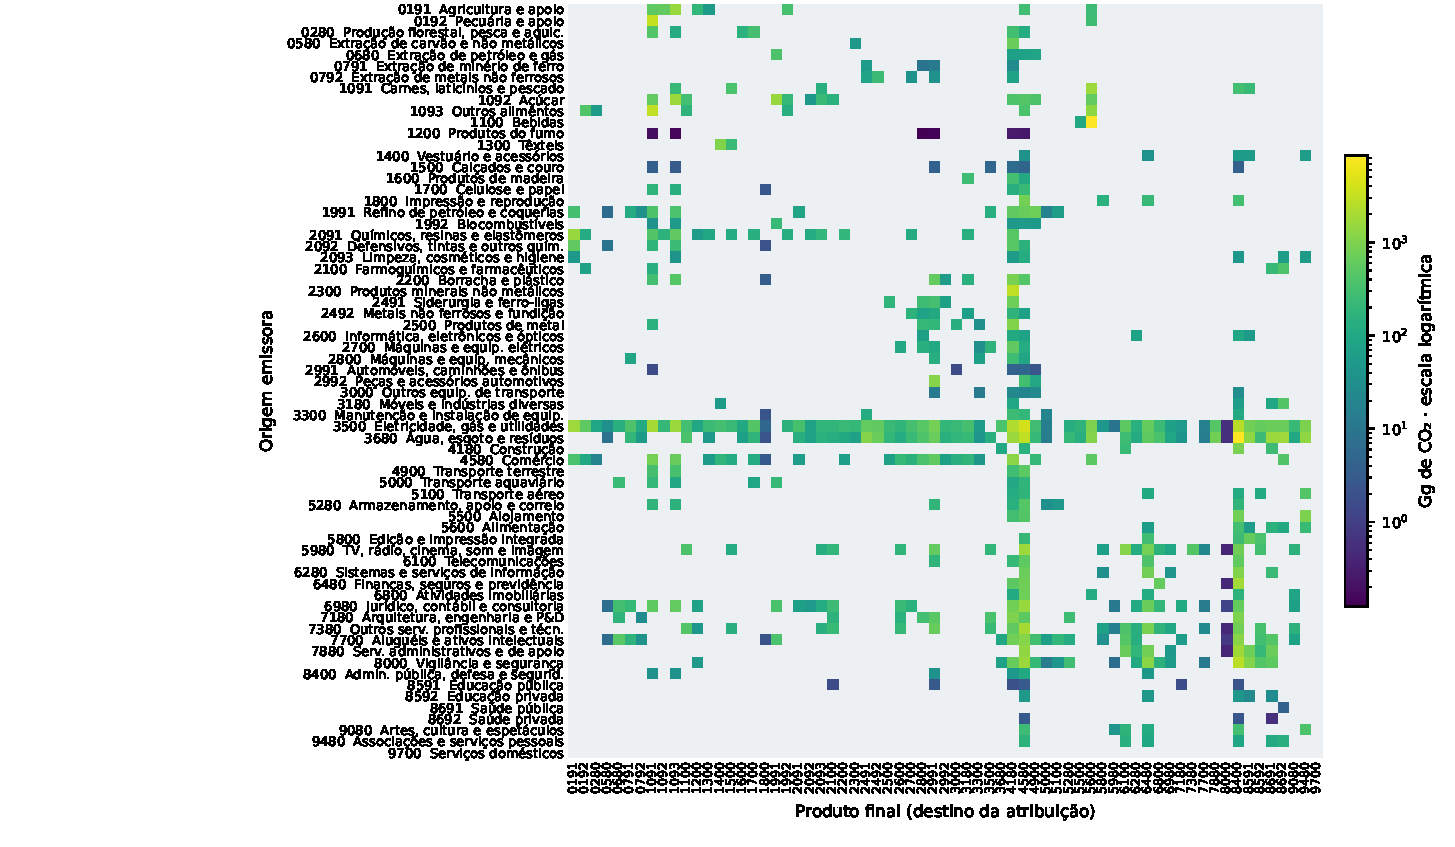
\includegraphics[width=\linewidth,height=0.68\textheight,keepaspectratio]{figuras/matriz_peso.pdf}
\begin{notas}
Nota: cada linha identifica uma atividade emissora e cada coluna, o setor de um produto final. Cada célula colorida representa emissões da origem atribuídas ao destino, incluindo requisitos diretos e indiretos da produção nacional para a demanda doméstica e as exportações; emissões estrangeiras são excluídas. O filtro de disparidade retém a relação se ela é selecionada na perspectiva da origem ou do destino, preservando seu peso original na rede completa $W$. São representadas 575 relações, correspondentes a 70,69\% das emissões intersetoriais de $W$.
\par
A cor mede o volume atribuído à relação, em Gg de CO\textsubscript{2} (mil toneladas): azul claro indica menores volumes e azul escuro, maiores volumes. A escala é logarítmica; intervalos iguais entre as marcas da barra correspondem a multiplicações por dez. As cores não são normalizadas por linha ou coluna e não medem intensidade emissora ou concentração setorial. Cinza indica ausência no backbone, o que não implica necessariamente atribuição nula em $W$. A diagonal é excluída.
\par
Todas as 67 atividades permanecem nos eixos, na ordem do IBGE, com nomes abreviados nas linhas e códigos nas colunas. Os rótulos em negrito destacam as origens energia (3500) e água/resíduos (3680) e o destino construção (4180), examinados nas seções anteriores; não representam outra seleção de relações.
\par
Dados: Matriz de Insumo-Produto do IBGE de 2015 e coeficientes de emissão interpolados de \textcite{sanguinetAzzoni2024}.
\end{notas}
\end{figure}
\end{landscape}

\subsection{Importância local nas duas perspectivas da relação}

Os perfis completos mostram como os pesos se distribuem; o filtro acrescenta a avaliação da importância local de cada relação para suas duas extremidades. As cores da Figura~\ref{fig:rede-focos} evidenciam o predomínio de saídas no recorte de energia e de entradas no de construção, mantendo as demais relações do mesmo backbone ao fundo. O motivo da retenção e a cobertura, apresentados na Tabela~\ref{tab:motivos-casos} e nos painéis do \ref{anexo:paineis}, permitem interpretar essa diferença entre as duas vistas.

\begin{table}[htbp]
\centering
\caption{Motivos de retenção e cobertura nos recortes de energia e construção.}
\label{tab:motivos-casos}
\small
\begin{tabular}{@{}lrrrrr@{}}
\toprule
Recorte & Arestas & Só saída & Só entrada & Ambos & Cobertura (\%) \\
\midrule
Energia: entradas & 7 & 1 & 5 & 1 & 42,1 \\
Energia: saídas & 62 & 0 & 56 & 6 & 99,2 \\
Construção: entradas & 45 & 41 & 0 & 4 & 91,4 \\
Construção: saídas & 5 & 4 & 1 & 0 & 57,0 \\
\bottomrule
\end{tabular}
\begin{notas}
Nota: $\alpha=0{,}05$. Saída e entrada nas colunas de motivo identificam o teste na origem e no destino da aresta, independentemente da atividade em destaque. Cobertura: peso retido dividido pela força da mesma atividade e direção em $W$. Os recortes compartilham arestas e não devem ser somados para obter totais da rede.
\end{notas}
\end{table}

Em energia, 56 das 62 saídas retidas passam somente pelo teste de entrada no destino. Energia tem participação destacada na composição externa de muitas demandas finais, embora cada destino possa representar parcela pequena das emissões distribuídas pela origem. Por exemplo, energia $\rightarrow$ alimentação (5600) representa 3,00\% das saídas externas de energia e 4,86\% das entradas externas de alimentação. A relação é selecionada somente na perspectiva do destino, evidenciando a diferença entre a composição recebida por uma atividade e a distribuição das emissões pela outra.

Em construção, 41 das 45 entradas passam somente pelo teste de saída na origem. Construção representa parcela destacada das atribuições externas dessas origens, mesmo quando a contribuição individual é pequena no total recebido pelo destino. Produtos de metal (2500) $\rightarrow$ construção, por exemplo, corresponde a 32,57\% das saídas externas da origem e a 4,42\% das entradas externas do destino. O filtro retém essa ligação somente pelo teste de saída na origem. Ela identifica uma demanda final que concentra parte expressiva das atribuições externas de produtos de metal, mesmo ocupando uma posição menor na composição recebida por construção.

As entradas de construção selecionadas pelos dois testes vêm de produtos de minerais não metálicos, energia, água/resíduos e comércio. A relação energia $\rightarrow$ construção, comum aos dois recortes, pesa aproximadamente 2\,263 Gg: 7,23\% das saídas externas de energia e 9,64\% das entradas externas de construção. Sua seleção nas duas extremidades conecta os papéis predominantes dos dois casos.

As saídas de energia e as entradas de construção têm as maiores coberturas dos respectivos recortes (Tabela~\ref{tab:motivos-casos}). Nas direções inversas, as listas curtas não autorizam desprezar as relações omitidas em conjunto. Tampouco a diferença entre 62 saídas de energia e 45 entradas de construção indica concentração distinta: na rede completa, os respectivos números efetivos são próximos, ambos de 20,8 contrapartes.

A sensibilidade qualifica a leitura desses papéis. Entre $\alpha=0{,}01$ e $0{,}10$, energia mantém de 54 a 64 saídas, com cobertura de 92,12\% a 99,96\%, enquanto construção mantém de 32 a 55 entradas, com cobertura de 74,31\% a 97,76\% (Tabela~\ref{tab:sensibilidade-casos}). Em todos os parâmetros, predomina o teste somente de entrada no destino nas saídas de energia e somente de saída na origem nas entradas de construção. Os cinco maiores destinos de energia permanecem selecionados. Esses resultados sustentam a leitura dos papéis ilustrados dentro da faixa examinada, apesar das mudanças no número de ligações e na cobertura.

A permanência de cada relação, contudo, exige verificação própria. Entre as cinco maiores origens de construção, água/resíduos deixa de ser selecionada em $\alpha=0{,}01$, embora represente 6,78\% do perfil externo recebido. Energia $\rightarrow$ construção permanece selecionada pelos dois testes nos três parâmetros. A composição da rede completa e os saldos não mudam com $\alpha$; a instabilidade de uma ligação no backbone delimita sua seleção sob o modelo nulo, sem alterar o volume de sua atribuição.



\clearpage
\begin{figure}[p]
\centering
\caption{Duas perspectivas do mesmo backbone: (a) destaque para energia (3500).}
\label{fig:rede-focos}
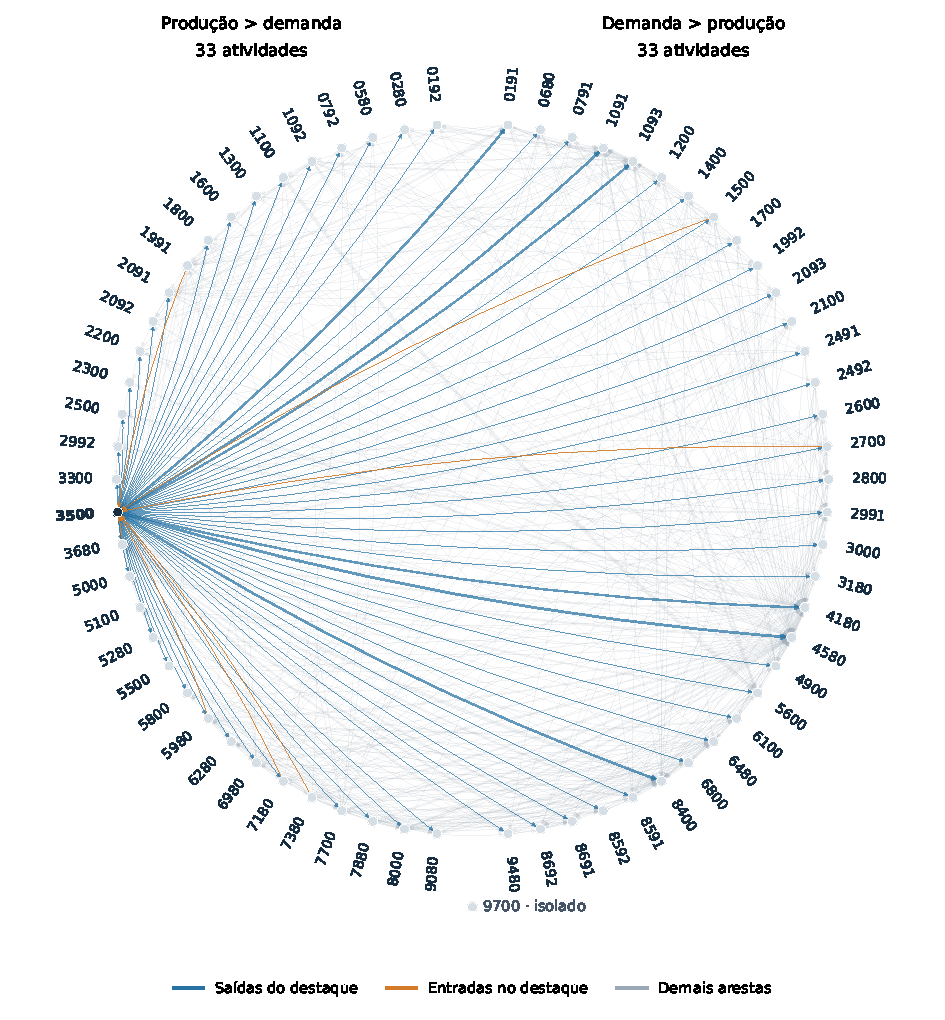
\includegraphics[width=\textwidth,height=0.76\textheight,keepaspectratio]{figuras/rede_foco_3500.pdf}
\begin{notas}
Nota: Cada vista mantém 67 nós e 575 arestas em $\alpha=0{,}05$. Azul: saídas do destaque; laranja: entradas; cinza: demais arestas. Energia tem 62 saídas e sete entradas, com cobertura de 99,2\% e 42,1\% do volume externo de cada direção. Área dos nós uniforme; espessura cresce com a raiz quadrada do peso. Posição definida pelo sinal de $u-c$ e pela ordem IBGE: 33 nós com $c>u$ à esquerda, 33 com $u>c$ à direita e o isolado abaixo. A disposição não resulta de centralidade ou comunidade.
\end{notas}
\end{figure}
\clearpage
\begin{figure}[p]
\ContinuedFloat
\centering
\caption{Duas perspectivas do mesmo backbone: (b) destaque para construção (4180).}
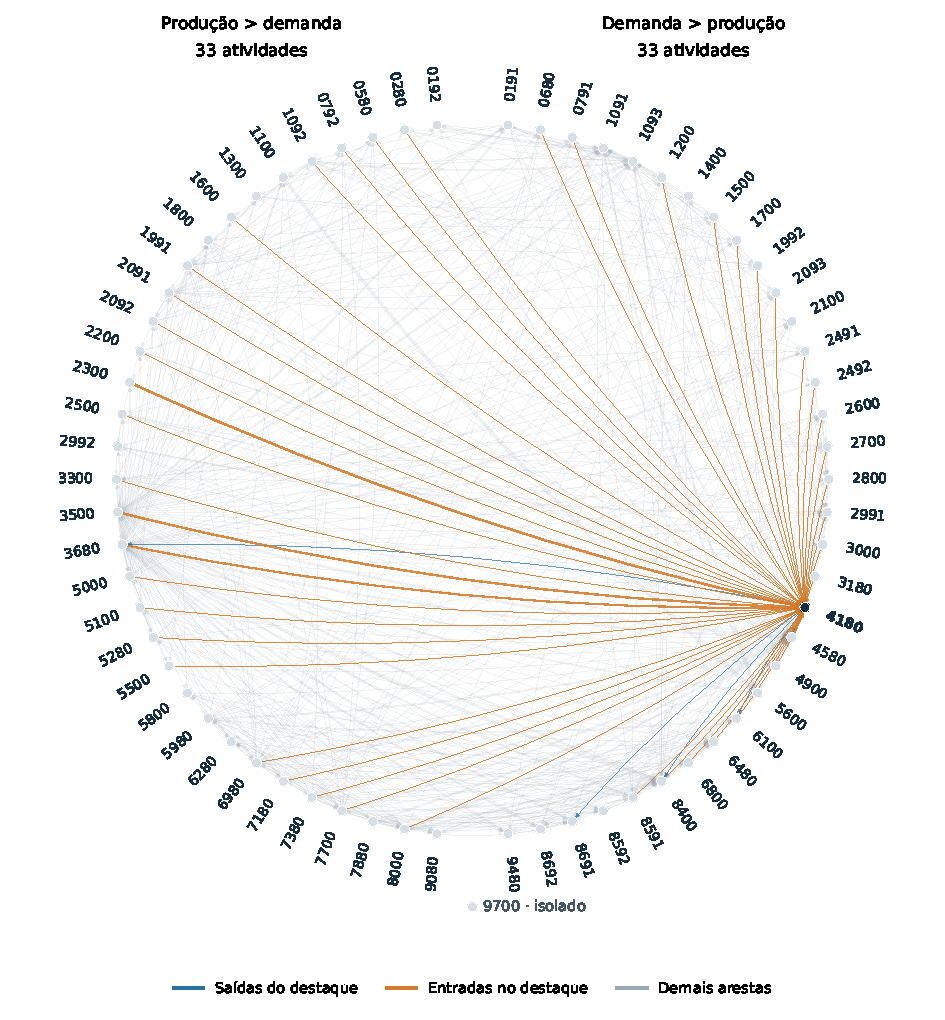
\includegraphics[width=\textwidth,height=0.76\textheight,keepaspectratio]{figuras/rede_foco_4180.pdf}
\begin{notas}
Nota: Mesmos nós, arestas, posições e escala de espessura do painel (a). Construção tem cinco saídas e 45 entradas, com cobertura de 57,0\% e 91,4\%. Cores representam direção em relação ao destaque, não motivo de retenção. As duas vistas preservam 70,69\% do peso intersetorial de $W$. Cruzamentos e proximidade não representam trajetórias ou distâncias econômicas; relações individuais podem ser consultadas na matriz e nos painéis do anexo.
\end{notas}
\end{figure}
\clearpage
